\documentclass[a4paper,12pt]{mwart}
\usepackage{graphicx}
\usepackage{amsmath,amsfonts,amsthm,amssymb,mathtools}
\usepackage{polski}
\usepackage{dirtree}
\usepackage[colorlinks=true, urlcolor=blue, linkcolor=red]{hyperref}
\usepackage{outlines}
\usepackage{minted}
\usepackage{xcolor}
\graphicspath{{../obrazy/}} %configuring the graphicx package

\definecolor{LightGray}{gray}{0.92}

\title{Dokumentacja projektu z baz danych}
\author{
    Jan Lewandowski, \and
    Szymon Jończak-Lis, \and
    Cezary Czetyrba, \and
    Michał Mickiewicz \\[1ex]
}
\date{20.01.2025}


\begin{document}
\maketitle

\section{Spis użytych technologii}

\begin{outline}
    \1 Python
        \2 wersja $>= 3.9$
        \2 moduły:
            \3 pandas
            \3 mysql-connector-python
            \3 python-dotenv
    \1 R
        \2 wersja $>= 4.4.2$
        \2 pakiety:
            \3 RMariaDB
            \3 ggplot2
            \3 ggrepel
            \3 lattice
            \3 dplyr
            \3 tidyverse
            \3 ggpubr
    \1 RStudio
        \2 wersja $>=$ \begin{verbatim}2024.12.0+467\end{verbatim}
    \1 Visual Studio Code
        \2 Dodatki
            \3 ERD editor
            \3 Inline SQL
    \1 Git, GitHub
    \1 Git Bash w systemie Windows
\end{outline}

\newpage

\section{Struktura projektu}

\dirtree{%
    .1 /.
    .2 .github/.
    .2 dane\_statystyczne/.
    .3 Imiona\_nadane\_dzieciom\_w\_Polsce\_w\_*.csv.
    .3 nazwiska\_meskie.csv.
    .3 nazwiska\_zenskie.csv.
    .2 dokumentacja/.
    .3 dokumentacja.pdf.
    .3 dokumentacja.tex.
    .3 schemat\_bazy\_danych.vuerd.
    .2 obrazy/.
    .3 baza\_danych\_fullsize.png.
    .3 baza\_danych.png.
    .2 raport/.
    .3 raport.html.
    .3 raport.pdf.
    .3 raport.Rmd.
    .2 wypelnienie/.
    .3 custom\_util.py.
    .3 do\_wypelnienia.py.
    .3 sql.py.
    .3 wypelnienie.py.
    .2 .env.example.
    .2 .gitignore.
    .2 LICENSE.
    .2 README.md.
    .2 requirements.txt.
}

\hspace{1cm}

\noindent Projekt podzielony jest na główne foldery i pliki:

\begin{outline}
    \1 \textbf{.github}
        \2 Folder zawierający pliki konfiguracyjne dla GitHub Actions. W naszym przypadku jest to analiza stylistyczna kodu.
    \1 \textbf{dane\_statystyczne}
        \2 Folder zawierający pliki z danymi statystycznymi. Są to pliki CSV z imionami i nazwiskami.
            \3 Źródła:
                \4 \href{https://dane.gov.pl/en/dataset/1681,nazwiska-osob-zyjacych-wystepujace-w-rejestrze-pesel}{Nazwiska w rejestrze PESEL}
                \4 \href{https://dane.gov.pl/en/dataset/219,imiona-nadawane-dzieciom-w-polsce}{Imiona nadane dzieciom w Polsce}
    \1 \textbf{dokumentacja}
        \2 Folder zawierający pliki z dokumentacją projektu. Znajduje się tam plik \texttt{dokumentacja.pdf}, który jest wygenerowany z pliku \texttt{dokumentacja.tex} oraz \texttt{schemat\_bazy\_danych.vuerd} zawierający schemat bazy danych w formacie ERD Editor. 
    \1 \textbf{obrazy}
        \2 Folder zawierający obrazy wykorzystane w raporcie oraz dokumentacji. 
    \1 \textbf{raport}
        \2 Folder zawierający pliki z raportem projektu. Znajdują się tam pliki \texttt{raport.pdf} oraz \texttt{raport.html}, które są generowane z pliku \texttt{raport.Rmd}.
    \1 \textbf{wypelnienie}
        \2 Folder zawierający skrypty do wypełnienia bazy danych. Znajduje się tam główny plik \texttt{wypelnienie.py}, który wypełnia bazę danych.
            \3 \texttt{custom\_util.py} - plik z funkcjami pomocniczymi.
            \3 \texttt{do\_wypelnienia.py} - plik z danymi na temat wycieczek i pracowników.
            \3 \texttt{sql.py} - plik z zapytaniami SQL.
    \1 \textbf{.env.example}
        \2 Przykładowy plik środowiskowy.
    \1 \textbf{.gitignore}
        \2 Lista plików ignorowanych przez Git.
    \1 \textbf{LICENSE}
        \2 Licencja projektu.
    \1 \textbf{README.md}
        \2 Ogólny opis projektu.
\end{outline}


\section{Instrukcja uruchomienia}

Aby uruchomić projekt potrzebny jest Python w wersji 3.9 lub nowszej. Po sklonowaniu repozytorium należy zainstalować wymagane moduły Pythona:

\begin{minted}[
    frame=lines,
    framesep=2mm,
    baselinestretch=1.2,
    bgcolor=LightGray,
    fontsize=\footnotesize,
    linenos,
    framesep=10pt
    ]{bash}
cd projekt-bazy-danych
pip install -r requirements.txt
\end{minted}

Następnie należy skopiować plik \texttt{.env.example} i zmienić jego nazwę na \texttt{.env}. W pliku tym należy podać hasło do połączenia z bazą danych.

\begin{minted}[
    frame=lines,
    framesep=2mm,
    baselinestretch=1.2,
    bgcolor=LightGray,
    fontsize=\footnotesize,
    linenos,
    framesep=10pt
    ]{bash}
cp .env.example .env
vim .env
\end{minted}

Po zainstalowaniu modułów i uzupełnieniu pliku \texttt{.env} można uruchomić skrypt wypełniający bazę danych.

\begin{minted}[
    frame=lines,
    framesep=2mm,
    baselinestretch=1.2,
    bgcolor=LightGray,
    fontsize=\footnotesize,
    linenos,
    framesep=10pt
    ]{bash}
python wypelnienie/wypelnienie.py
\end{minted}

Kiedy zakończy się on poprawnie wypisując \texttt{Wypelniono baze danych}, możemy wygenerować raport. Można go otworzyć w \texttt{RStudio} i uruchomić przyciskiem \texttt{Knit} lub mając \texttt{Rscript} i \texttt{pandoc} poprzez umieszczenie 

\begin{minted}[
    frame=lines,
    framesep=2mm,
    baselinestretch=1.2,
    bgcolor=LightGray,
    fontsize=\footnotesize,
    linenos,
    framesep=10pt
    ]{bash}
export PATH=$PATH:"C:\Program Files\R\R-4.4.2\bin\x64"
export PATH=$PATH:"C:\Program Files\RStudio\resources\app
\bin\quarto\bin\tools"
\end{minted}

\noindent w \texttt{$\sim$/.bashrc} gdy używamy \texttt{Git Bash}. Po dodaniu zmiennych do ścieżki należy odświeżyć konsolę. Raport można wtedy wygenerować komendą

\begin{minted}[
    frame=lines,
    framesep=2mm,
    baselinestretch=1.2,
    bgcolor=LightGray,
    fontsize=\footnotesize,
    linenos,
    framesep=10pt
    ]{bash}
Rscript -e 'rmarkdown::render("raport/raport.Rmd")'
\end{minted}

Teraz możemy obejrzeć gotowy raport, znajduje się od w pliku \newline \texttt{raport/raport.pdf}.

\section{Schemat bazy danych}
\begin{figure}[h!]
    \centering
    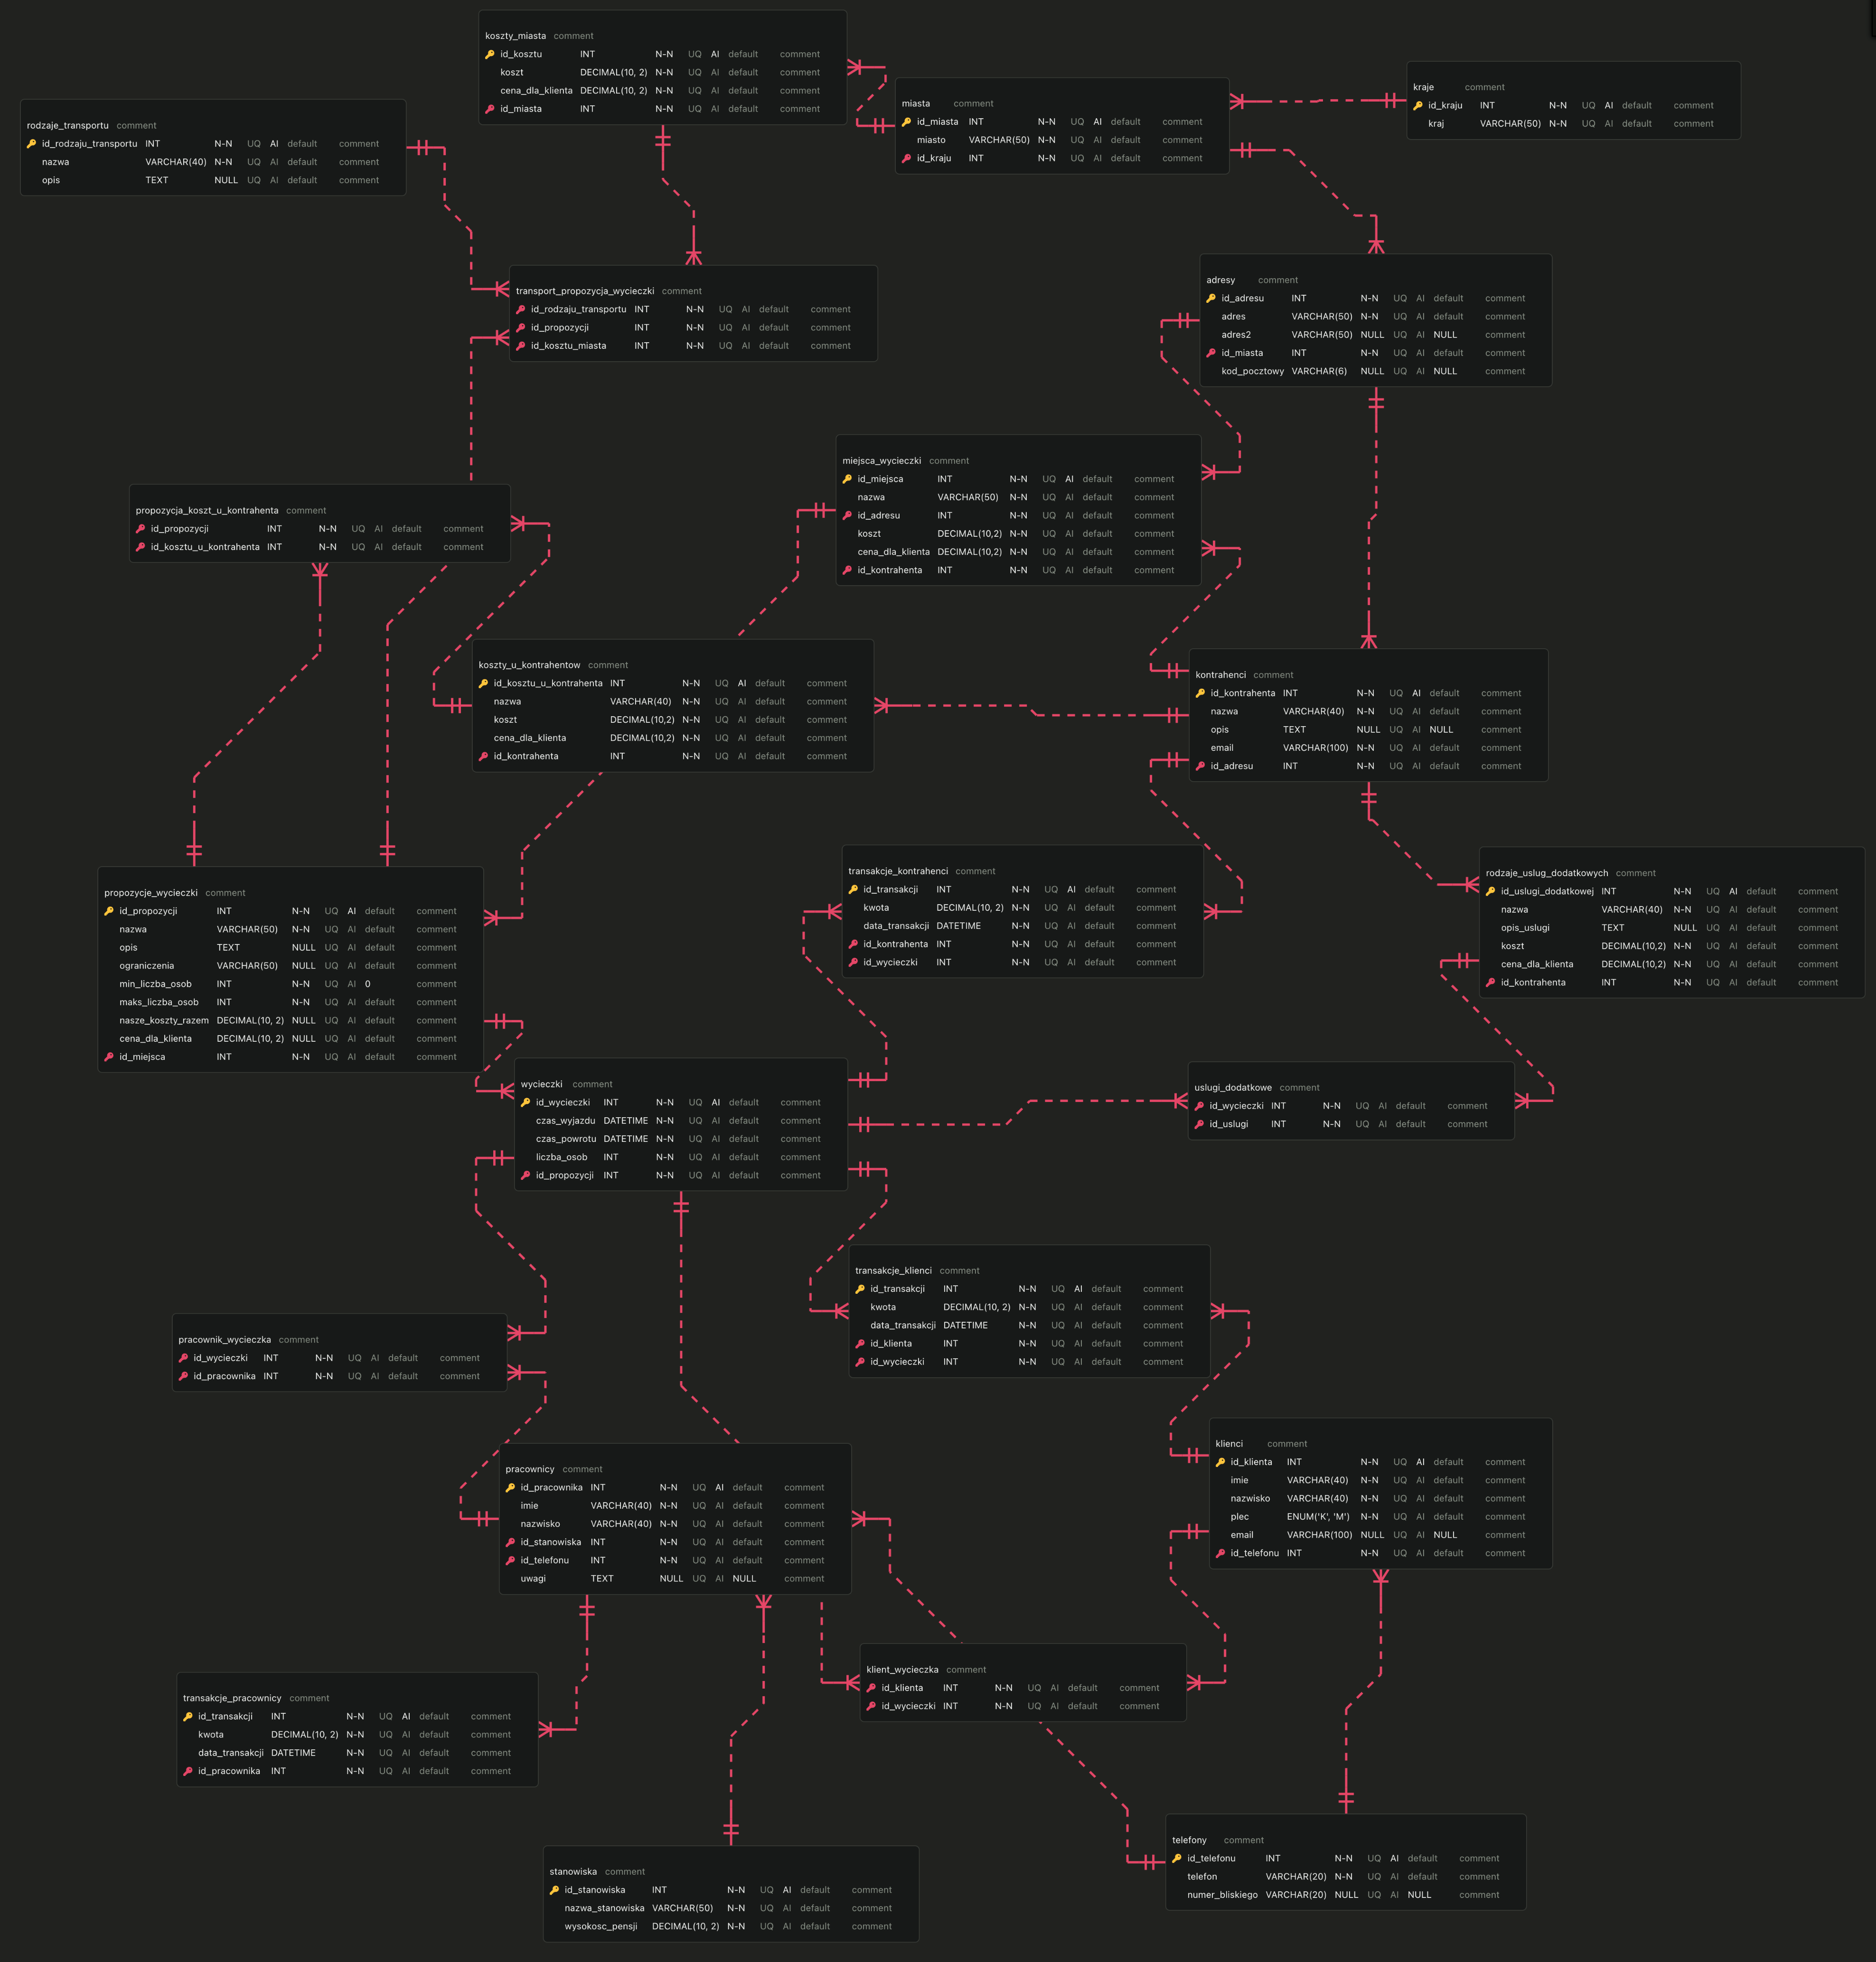
\includegraphics[width=0.9\textwidth]{baza_danych_fullsize.png}
    \caption{Schemat bazy danych}
\end{figure}
\section{Analiza tabel}
\subsection{Tabela rodzaje\_transportu}
Tabela jest postaci:

rodzaje\_transportu(\underline{id\_rodzaju\_transportu}, nazwa, opis)

\noindent Jedynymi nietrywialnymi zależnościami funkcyjnymi są:
$$   id\_rodzaju\_transportu  \rightarrow nazwa $$
$$   id\_rodzaju\_transportu  \rightarrow opis$$
Zatem każda nietrywialna zależność funkcyjna zaczyna się od nadklucza i tabela  spełnia wymagania bycia w EKNF.

\subsection{Tabela koszty\_miasta}
Tabela jest postaci:

koszty\_miasta(\underline{id\_kosztu\_miasta}, koszt, cena\_dla\_klienta, id\_miasta)

\noindent Jedynymi nietrywialnymi zależnościami funkcyjnymi są:
$$   id\_kosztu\_miasta  \rightarrow koszt $$
$$   id\_kosztu\_miasta  \rightarrow cena\_dla\_klienta $$
$$   id\_kosztu\_miasta  \rightarrow id\_miasta $$

Zatem każda nietrywialna zależność funkcyjna zaczyna się od nadklucza i tabela  spełnia wymagania bycia w EKNF.

\subsection{Tabela miasta}
Tabela jest postaci:

miasta(\underline{id\_miasta}, miasto, id\_kraju)

\noindent Jedynymi nietrywialnymi zależnościami funkcyjnymi są:
$$   id\_miasta  \rightarrow miasto $$
$$   id\_miasta  \rightarrow id\_kraju $$
Zakładamy, że miasto nie definiuje jednoznacznie kraju.
Zatem każda nietrywialna zależność funkcyjna zaczyna się od nadklucza i tabela  spełnia wymagania bycia w EKNF.

\subsection{Tabela kraje}
Tabela jest postaci:

kraje(\underline{id\_kraju}, kraj)

\noindent Jedyną nietrywialną zależnością funkcyjną jest:
$$   id\_kraju  \rightarrow kraj$$


Zatem każda nietrywialna zależność funkcyjna zaczyna się od nadklucza i tabela  spełnia wymagania bycia w EKNF.

\subsection{Tabela transport\_propozycja\_wycieczki}
Tabela jest postaci:

transport\_propozycja\_wycieczki(id\_rodzaju\_transportu, id\_propozycji, id\_kosztu\_miasta)

W tej tabeli nie występują nietrywialne zależności funkcyjne, wszystkie trzy kolumny tworzą klucz elementarny, a pomiędzy nimi nie ma zależności.
Zatem każda nietrywialna zależność funkcyjna zaczyna się od nadklucza i tabela  spełnia wymagania bycia w EKNF.

\subsection{Tabela adresy}
Tabela jest postaci:

adresy(\underline{id\_adresu}, adres, adres2, id\_miasta, kod\_pocztowy)

\noindent Jedynymi nietrywialnymi zależnościami funkcyjnymi są:
$$   id\_adresu  \rightarrow adres $$
$$   id\_adresu  \rightarrow adres2 $$
$$   id\_adresu  \rightarrow id\_miasta $$
$$   id\_adresu  \rightarrow kod\_pocztowy $$
Zakładamy, że kod pocztowy nie definiuje jednoznacznie miasta i  adres nie definiuje kodu pocztowego.


Zatem każda nietrywialna zależność funkcyjna zaczyna się od nadklucza i tabela  spełnia wymagania bycia w EKNF.


\subsection{Tabela miejsca\_wycieczki}
Tabela jest postaci:

miejsca\_wycieczki(\underline{id\_miejsca}, nazwa, id\_adresu, koszt, cena\_dla\_klienta, id\_kontrahenta)

\noindent Jedynymi nietrywialnymi zależnościami funkcyjnymi są:
$$   id\_miejsca  \rightarrow nazwa $$
$$   id\_miejsca  \rightarrow id\_adresu $$
$$   id\_miejsca  \rightarrow koszt $$
$$   id\_miejsca  \rightarrow cena\_dla\_klienta $$
$$   id\_miejsca  \rightarrow id\_kontrahenta $$


Zatem każda nietrywialna zależność funkcyjna zaczyna się od nadklucza i tabela  spełnia wymagania bycia w EKNF.

\subsection{Tabela propozycja\_koszt\_u\_kontrahenta}
Tabela jest postaci:

propozycja\_koszt\_u\_kontrahenta(id\_propozycji, id\_kosztu\_u\_kontrahenta)

W tej tabeli nie występują nietrywialne zależności funkcyjne, wszystkie trzy kolumny tworzą klucz elementarny, a pomiędzy nimi nie ma zależności.
Zatem każda nietrywialna zależność funkcyjna zaczyna się od nadklucza i tabela  spełnia wymagania bycia w EKNF.


\subsection{Tabela koszty\_u\_kontrahenta}
Tabela jest postaci:

koszty\_u\_kontrahenta(\underline{id\_kosztu\_u\_kontrahenta}, nazwa, koszt, cena\_dla\_klienta, id\_kontrahenta)

\noindent Jedynymi nietrywialnymi zależnościami funkcyjnymi są:
$$   id\_kosztu\_u\_kontrahenta\rightarrow nazwa $$
$$   id\_kosztu\_u\_kontrahenta\rightarrow koszt $$
$$   id\_kosztu\_u\_kontrahenta\rightarrow cena\_dla\_klienta $$
$$   id\_kosztu\_u\_kontrahenta\rightarrow id\_kontrahenta $$


Zatem każda nietrywialna zależność funkcyjna zaczyna się od nadklucza i tabela  spełnia wymagania bycia w EKNF.


\subsection{Tabela kontrahenci}
Tabela jest postaci:

kontrahenci(\underline{id\_kontrahenta}, nazwa, opis, email, id\_adresu)

\noindent Jedynymi nietrywialnymi zależnościami funkcyjnymi są:
$$   id\_kontrahenta  \rightarrow nazwa $$
$$   id\_kontrahenta  \rightarrow opis $$
$$   id\_kontrahenta \rightarrow email $$
$$   id\_kontrahenta \rightarrow id\_adresu $$


Zatem każda nietrywialna zależność funkcyjna zaczyna się od nadklucza i tabela  spełnia wymagania bycia w EKNF.


\subsection{Tabela propozycje\_wycieczki}
Tabela jest postaci:

propozycje\_wycieczki(\underline{id\_propozycji}, nazwa, opis, ograniczenia, min\_liczba\_osob, max\_liczba\_osob, nasze\_koszty\_razem, cena\_dla\_klienta, id\_miejsca)

\noindent Jedynymi nietrywialnymi zależnościami funkcyjnymi są:
$$   id\_propozycji  \rightarrow nazwa $$
$$   id\_propozycji\rightarrow opis $$
$$   id\_propozycji\rightarrow ograniczenia $$
$$   id\_propozycji\rightarrow min\_liczba\_osob $$
$$   id\_propozycji\rightarrow max\_liczba\_osob $$
$$   id\_propozycji\rightarrow nasze\_koszty\_razem $$
$$   id\_propozycji\rightarrow cena\_dla\_klienta $$
$$   id\_propozycji\rightarrow id\_miejsca $$


Zatem każda nietrywialna zależność funkcyjna zaczyna się od nadklucza i tabela  spełnia wymagania bycia w EKNF.

\subsection{Tabela wycieczki}
Tabela jest postaci:

wycieczki(\underline{id\_wycieczki}, czas\_wyjazdu, czas\_powrotu, liczba\_osob, id\_propozycji)

\noindent Jedynymi nietrywialnymi zależnościami funkcyjnymi są:
$$   id\_wycieczki\rightarrow czas\_wyjazdu$$
$$   id\_wycieczki\rightarrow czas\_powrotu $$
$$   id\_wycieczki\rightarrow liczba\_osob $$
$$   id\_wycieczki\rightarrow id\_propozycji $$


Zatem każda nietrywialna zależność funkcyjna zaczyna się od nadklucza i tabela  spełnia wymagania bycia w EKNF.

\subsection{Tabela transakcje\_kontrahenci}
Tabela jest postaci:

transakcje\_kontrahenci(\underline{id\_transakcji}, kwota, data\_transakcji, id\_kontrahenta, id\_wycieczki)

\noindent Jedynymi nietrywialnymi zależnościami funkcyjnymi są:
$$   id\_transakcji\rightarrow kwota $$
$$   id\_transakcji\rightarrow czas\_wyjazdu$$
$$   id\_transakcji\rightarrow data\_transakcji $$
$$   id\_transakcji\rightarrow id\_kontrahenta $$
$$   id\_transakcji\rightarrow id\_wycieczki$$

Zatem każda nietrywialna zależność funkcyjna zaczyna się od nadklucza i tabela  spełnia wymagania bycia w EKNF.

\subsection{Tabela rodzaje\_uslug\_dodatkowych}
Tabela jest postaci:

 rodzaje\_uslug\_dodatkowych(\underline{id\_uslugi\_dodatkowej}, nazwa, opis\_uslugi, koszt, cena\_dla\_klienta, id\_kontrahenta)

\noindent Jedynymi nietrywialnymi zależnościami funkcyjnymi są:
$$   id\_uslugi\_dodatkowej\rightarrow nazwa $$
$$   id\_uslugi\_dodatkowej\rightarrow opis\_uslugi$$
$$   id\_uslugi\_dodatkowej\rightarrow koszt$$
$$   id\_uslugi\_dodatkowej\rightarrow cena\_dla\_klienta $$
$$   id\_uslugi\_dodatkowej\rightarrow id\_kontrahenta$$

Zatem każda nietrywialna zależność funkcyjna zaczyna się od nadklucza i tabela  spełnia wymagania bycia w EKNF.


\subsection{Tabela uslugi\_dodatkowe}
Tabela jest postaci:

uslugi\_dodatkowe(id\_wycieczki, id\_uslugi)

W tej tabeli nie występują nietrywialne zależności funkcyjne, dwie kolumny  tworzą klucz elementarny, a pomiędzy nimi nie ma zależności.
Zatem każda nietrywialna zależność funkcyjna zaczyna się od nadklucza i tabela  spełnia wymagania bycia w EKNF.

\subsection{Tabela pracownik\_wycieczka}
Tabela jest postaci:

pracownik\_wycieczka(id\_wycieczki, id\_pracownika)

W tej tabeli nie występują nietrywialne zależności funkcyjne, dwie kolumny  tworzą klucz elementarny, a pomiędzy nimi nie ma zależności.
Zatem każda nietrywialna zależność funkcyjna zaczyna się od nadklucza i tabela  spełnia wymagania bycia w EKNF.

\subsection{Tabela pracownicy}
Tabela jest postaci:

pracownicy(\underline{id\_pracownika}, imie, nazwisko, id\_stanowiska, id\_telefonu, uwagi)

\noindent Jedynymi nietrywialnymi zależnościami funkcyjnymi są:
$$   id\_pracownika\rightarrow imie $$
$$   id\_pracownika\rightarrow nazwisko $$
$$   id\_pracownika\rightarrow id\_stanowiska $$
$$   id\_pracownika\rightarrow id\_telefonu $$
$$   id\_pracownika\rightarrow uwagi $$
Zakładamy, że imię i nazwisko nie identyfikują jednoznacznie pracownika.
Skoro każda nietrywialna zależność funkcyjna zaczyna się od nadklucza i tabela  spełnia wymagania bycia w EKNF.


\subsection{Tabela telefony}
Tabela jest postaci:

telefony(\underline{id\_telefonu}, telefon, numer\_bliskiego)

\noindent Jedynymi nietrywialnymi zależnościami funkcyjnymi są:
$$   id\_telefonu \rightarrow telefon $$
$$   id\_telefonu \rightarrow numer\_bliskiego $$
Zakładamy, że numery telefonów nie są unikalne,
zatem każda nietrywialna zależność funkcyjna zaczyna się od nadklucza i tabela  spełnia wymagania bycia w EKNF.

\subsection{Tabela stanowiska}
Tabela jest postaci:

stanowiska(\underline{id\_stanowiska}, nazwa\_stanowiska, wysokosc\_pensji)

\noindent Jedynymi nietrywialnymi zależnościami funkcyjnymi są:
$$   id\_stanowiska \rightarrow nazwa\_stanowiska $$
$$   id\_stanowiska \rightarrow wysokosc\_pensji $$
Zakładamy, że nie ma zależności, które zaczynają się od stanowiska,
zatem każda nietrywialna zależność funkcyjna zaczyna się od nadklucza i tabela  spełnia wymagania bycia w EKNF.

\subsection{Tabela klient\_wycieczka}
Tabela jest postaci:

klient\_wycieczka(id\_wycieczki, id\_klienta)

W tej tabeli nie występują nietrywialne zależności funkcyjne, dwie kolumny  tworzą klucz elementarny, a pomiędzy nimi nie ma zależności.
Zatem każda nietrywialna zależność funkcyjna zaczyna się od nadklucza i tabela  spełnia wymagania bycia w EKNF.



\subsection{Tabela transakcje\_pracownicy}
Tabela jest postaci:

transakcje\_pracownicy(\underline{id\_transakcji}, kwota, data\_transakcji, id\_pracowniak)

\noindent Jedynymi nietrywialnymi zależnościami funkcyjnymi są:
$$   id\_transakcji\rightarrow kwota $$
$$   id\_transakcji\rightarrow czas\_wyjazdu$$
$$   id\_transakcji\rightarrow data\_transakcji $$
$$   id\_transakcji\rightarrow id\_pracownika $$

Zatem każda nietrywialna zależność funkcyjna zaczyna się od nadklucza i tabela  spełnia wymagania bycia w EKNF.

\subsection{Tabela transakcje\_klienci}
Tabela jest postaci:

transakcje\_klienci(\underline{id\_transakcji}, kwota, data\_transakcji, id\_klienta, id\_wycieczki)

\noindent Jedynymi nietrywialnymi zależnościami funkcyjnymi są:
$$   id\_transakcji\rightarrow kwota $$
$$   id\_transakcji\rightarrow czas\_wyjazdu$$
$$   id\_transakcji\rightarrow data\_transakcji $$
$$   id\_transakcji\rightarrow id\_klienta $$
$$   id\_transakcji\rightarrow id\_wycieczki $$
Zatem każda nietrywialna zależność funkcyjna zaczyna się od nadklucza i tabela  spełnia wymagania bycia w EKNF.

\subsection{Tabela klienci}
Tabela jest postaci:

klienci(\underline{id\_klienta}, imie, nazwisko, plec, email, id\_telefonu)

\noindent Jedynymi nietrywialnymi zależnościami funkcyjnymi są:
$$   id\_klienta\rightarrow imie $$
$$   id\_klienta\rightarrow nazwisko$$
$$   id\_klienta\rightarrow plec$$
$$   id\_klienta\rightarrow email $$
$$   id\_klienta\rightarrow id\_telefonu $$
Zakładamy, że imię i nazwisko nie identyfikują jednoznacznie klienta.
Zatem każda nietrywialna zależność funkcyjna zaczyna się od nadklucza i tabela  spełnia wymagania bycia w EKNF.



W żadnym połączeniu tabel nie ma zależności tranzytywnych, każda tabela pojedynczo jest w EKNF, zatem to pokazuje, że cała baza danych jest w EKNF.

\section{Co było najtrudniejsze w realizacji projektu}

\begin{outline}
    \1 Dopasowanie realistycznych kosztów usług i podróży.
    \1 Aktualizacja wypełniania bazy danych po zmianach w schemacie.
\end{outline}

\end{document}
